\documentclass[11pt]{article}
\usepackage{geometry}
\geometry{a4paper, bottom=20mm, top=30mm, left=15mm, right=15mm}
\usepackage{pdfpages}
\usepackage{fancyhdr}
\pagestyle{fancy}
\setlength{\parindent}{0cm}
\setlength{\headheight}{14pt}
\usepackage{tocloft}
\usepackage{parskip}
\usepackage[export]{adjustbox}
\usepackage{float}
\usepackage{subfig}
\usepackage{graphicx}
\graphicspath{{../figures}}
\usepackage{amsmath,blkarray,booktabs,bigstrut, amssymb}
\usepackage{pythonhighlight}
\usepackage{outlines}
\usepackage{soul}
\usepackage[hidelinks]{hyperref}
\usepackage[backend=biber, style=ieee]{biblatex}
\addbibresource{references.bib}
\defbibheading{bibliography}{} % Hides the "References" title
\usepackage{url}
\setcounter{biburllcpenalty}{7000}
\setcounter{biburlucpenalty}{8000}
\widowpenalty10000
\clubpenalty10000
\setcounter{secnumdepth}{3}
\usepackage[newfloat]{minted}
\usepackage{caption}
\newenvironment{code}{\captionsetup{type=listing}}{}
\SetupFloatingEnvironment{listing}{name=Code Listing}
 
\begin{document}

\newgeometry{top=20mm}
\begin{titlepage}
	\begin{center}
		\begin{figure}
			
\includegraphics[right]{logo.png}
		\end{figure}
		\vspace*{1cm}
		\textsc{\large ENEL373: Digital Electronics and Devices}\\[0.5cm]
		\textsc{\Large University of Canterbury}\\[3.5cm]
		\linespread{1}
		{\Huge\bfseries{Development of a Reaction \\[0.3cm] Timer in VHDL}} \\
		\vspace*{2cm}
		{\Huge Philip Brand \textit{\Large(15776928)}\\\par}
		{\Huge Michael Brown \textit{\Large(48571923)}\\\par}
		{\Huge Boston Black \textit{\Large(24668421)}\\\par}
		\vspace*{3cm}
		{\LARGE \today}
	\end{center}
\end{titlepage}
\restoregeometry

\fancyhead{}
\fancyhead[L]{\small{ENEL373 - Reaction Timer Project}}
\fancyhead[R]{\small{\today}}

\pagenumbering{roman}

\renewcommand{\baselinestretch}{1.3}\normalsize
\setlength{\cftbeforesecskip}{0.3em}
\renewcommand{\cftsecleader}{\cftdotfill{\cftdotsep}}
\addcontentsline{toc}{section}{Contents}
\tableofcontents\thispagestyle{fancy}
\renewcommand{\baselinestretch}{1}\normalsize

\newpage
\pagenumbering{arabic}

\section{Introduction}
% Outline (in your own words) the project requirements and what you achieved

Human reaction time is the interval between a stimulus and the response to that stimulus. There are two main types of reaction time; simple and choice. Simple reaction involves reacting to a singular stimulus, while choice reaction involves choosing the correct response from multiple stimuli. This project aims to implement a simple reaction time recorder on an FPGA in VHDL.

The reaction stimulus test starts with three LCD dots that turn off sequentially with a random delay. Once the last dot turns off, the user must press a button to stop the timer. The delay is then displayed on 8 7-segment displays. The FPGA stores the reaction delays from the last three tests, and can display the fastest, slowest, and average reaction time. The stored times can be cleared by the user.

This report outlines the implementation of the reaction timer, along with the design methods used, testing of some of the components, and discusses issues encountered during the project.

\section{Design Summary}
% Summarise your design.

The FPGA reaction stimulus and response recording depends on five major components; the eight-digit counter, the ALU, the reaction stimulus countdown, the error display, and the output select and override. These components are shown in Figure \ref{project_structure}. Each of these components are enabled and disabled via a finite state machine.

\begin{figure}[H]
	\centering
	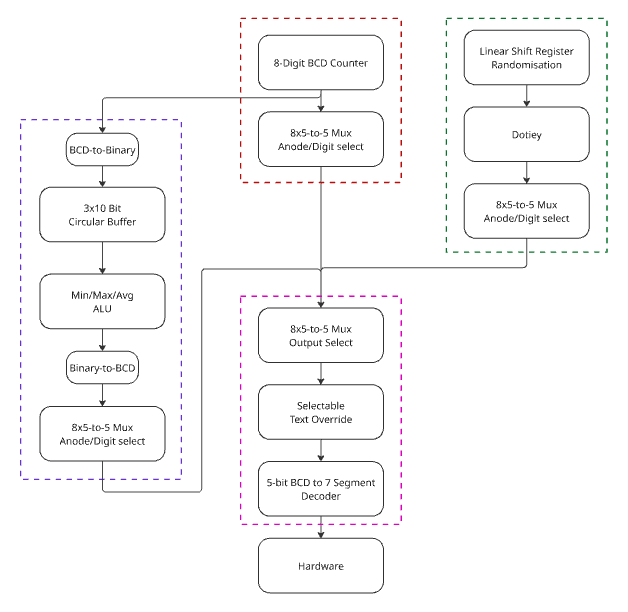
\includegraphics[width=0.66\textwidth]{project_overall_structure.png}
	\caption{Overview of VHDL reaction timer structure.}
	\label{project_structure}
\end{figure}

An eight-digit five-bit-BCD counter is the primary mechanism for keeping track of the reaction time in milliseconds for each stimulus test. Each BCD digit is passed into an 8x5-to-5 multiplexer. The purpose of this multiplexer is to synchronise the selected output digit with the seven segment display, meaning each digit is displayed on its respective display.

All BCD digits from the eight-digit counter are passed through the \texttt{bcd\_8\_to\_binary} component, which converts the BCD digits into a 28-bit binary number. The increased bus width is shown in Figure \ref{project_structure} as a thicker data transfer arrow. This binary number is then passed into a circular buffer which stores the reaction time data. The ALU reads the circular buffer to calculate the average, minimum, and maximum of the last three reaction times. These times are then converted back into BCD using the double dabble algorithm \cite{double_dabble}. Finally, another 8x5-to-5 multiplexer is used to select which digit to output to the display.

A linear feedback shift register is used to provide randomisation for each reaction stimulus countdown sequence. This shift register sets the upperbound for a clock divider, whose output triggers the shift register to change its pseudorandom output. The clock divider triggers each LCD dot during the countdown state, named \texttt{doitey}. The dots are then piped into the output to hardware select using another 8x5-to-5 multiplexer.

All four 8x5-to-5 multiplexers are piped into another 8x5-to-5 multiplexer used for seven segment output selection. This multiplexer selects which module to output depending on the active state. The multiplexer output is piped into a text override, which overwrites some of the digits with letters based on the active state. This is finally piped into the seven-segment decoder, which takes a five-bit BCD digit and converts it to an eight-bit seven-segment display light combination which is then piped to hardware.

% TODO: Review whether error state needs talking about

\section{Expanded Design Summary}
% (~2 pages): Describe the methods your group used to implement your FPGA design. Justify your final design. Support your descriptions and justifications with specific, explicit references to your VHDL source code in the appendix. VHDL descriptions could, for example, include an RTL description. 

\subsection{Design Methods}

The primary focus for the reaction timer project was to develop VHDL code that is easy to maintain and develop further. This led to a heavy focus on modular design and code reuse. Since the project was developed as a group, the other focus was for components to be developed and tested individually, and then put together with hopefully minimal issues.

\subsubsection{Diagramming}

The primary development method used in this project was to draw program or module flow diagrams before VHDL was written. These diagrams detailed the communication between individual components, and outlined the overall program structure. One such diagram is in Appendix C.

Clear communication of the expected inputs and outputs from each component between group members played a significant role in keeping the final assembly simple. One example of standard inputs/outputs is the use of five-bit BCD for all communication of characters or numbers. The only place five-bit BCD was not used for numbers was the ALU module.

\subsubsection{Naming and Syntax Conventions}

Another important aspect of the project ensuring high code quality, readability, and maintainability was strict rules around naming and syntax. This included consistent whitespace, indentation, case, and naming style. For example, all signals within an entity were postfixed with an underscore, and whether that signal was an input or an output. This can be seen in Code Listing \ref{code:entity_naming_convention} in Appendix A. This ensured when the components were used in the top-level Behavioural architecture with port mapping, it was easy to see which signals were inputs and outputs.

To make the difference between port and internal signals clear, port names were all capitalised, while internal signals were in all lowercase. The signal types were also capitalised for ports, e.g. \texttt{STD\_LOGIC}, instead of \texttt{std\_logic}. This can be seen in Code Listings \ref{code:case_io} and \ref{code:case} in Appendix A.

When naming components, an effort was made to name them in a way that described the capabilities of the component. For example,  \texttt{timer\_8\_num\_selectable} has eight numbers and one can be selected. The postfix \texttt{\_xb} was used to indicate a component had an \texttt{x} bit input or output. This is used in components such as \texttt{counter\_3b} and \texttt{decoder\_3b}.

\subsubsection{Component Reuse}

% TODO: Review why there is a section in italics?
In order to reduce the number of components requiring creation and maintenance, components were reused where possible. The most prominent example of this was the eight-channel five-bit multiplexer shown in Code Listing \ref{code:8x5_to_5_multiplexer} in Appendix A. The multiplexer took up to eight five-bit BCD inputs, and selected one of those to be output. The select lines and number of channels for the multiplexer corresponded with the segment display, allowing both to be controlled with the same signal. This capability made the multiplexer easy to use for displaying timer digits and error message characters. The same multiplexer was also used to select what output to pipe to the segment display, depending on the state. While not all multiplexer inputs were used in all instantiations, using the same component in all instances was logical as the component was known to work and integrate well with other components.

Another frequently reused component was the clock divider. The wide use of the component was aided by the ability for the upperbound to be set by an input rather than being hard-coded within the component, and the ability for upperbound to be updated during component use.  For example, the pseudorandom dot delay used the same \texttt{clk\_divider} component as real-time upperbound changes resulted in different clock speeds and therefore delays.

\subsubsection{Programming Techniques}

Another method used to implement the FPGA design was pair programming. This had to be done with care, as with three people working on the project, it would have been easy to leave one person out of the process, resulting in their lack of code understanding. However, pair programming did help ensure that minimal time was spent debugging, as the observer frequently caught subtleties of VHDL that the programmer missed. Pair programming was used to develop the circular buffer, counters, and FSM.

Since the project was significantly modularised, it was important that individual components could be developed and tested without hindering the development of other components. The method used to achieve this was git branching and merging. Individual components were developed on separate branches, tested, and then merged into the main branch. This ensured that the main branch was always stable, and that broken changes could be easily rolled back.

\subsection{Design Justification}

The reaction timer design is intended to allow easy modification or expansion. Keeping modularisation as a high priority during component design allowed each component to view the other components as a ``black box'', only interacting with each other through standardised interfaces. These interfaces were typically a single custom five-bit BCD data line, and were controlled by the generalised 8x5-to-5 multiplexer shown in Code Listing \ref{code:8x5_to_5_multiplexer} in Appendix A, reducing the required number of different components. The only exception to the five-bit data line was the output of the BCD counter, which output eight five-bit data lines simultaneously to the BCD-to-binary converter, as the converter operated on all digits at once. These eight data lines were put into a bus, as shown in Code Listing \ref{code:bcd_to_binary} in Appendix A.

A second benefit of each component being a ``black box'' was that since most components interacted through standardised interfaces, how the components operated internally was irrelevant. This allowed for significant changes within a component to how a task was completed, without disturbing inter-component communication, or the operation of other components.

The usage of the 8x5-to-5 multiplexer to select between outputs allows for the addition of states as desired by utilizing more multiplexer inputs, with output select lines controlled by the finite state machine. This is shown in Code Listing \ref{code:output_select_mux_instantiation} in Appendix A. If more states were to be added, then additional multiplexers can be connected for more input lines. This shows clear capability for design expansion.

A selectively enabled text override component was used to display text on the first two seven-segment displays, as this component centralised control of the text display. This further simplified other components by limiting their design to numeric manipulation, rather than alphabetic or alphanumeric manipulation.

% TODO: philip sir add justification of lfsr for randon number generation

\section{Module Testing}
% A brief section describing how you tested a significant module. Include at least one testbench and associated waveforms that demonstrate the functionality of a module in the report appendix.

% TODO: rename bcd_expanded_out, possibly remove just have a standard 4-bit output
% TODO: reorder waveform to be more logical - put alu output next to operation select and things like that, put clock at the top probably too
% TODO: add testbench waveform for BCD to binary converter

During development of the circular buffer, ALU, and associated data-type converters, the output numbers were too small. For example a minimum reaction time of 246 milliseconds would be displayed as 91 milliseconds. Since the delay would be displayed correctly immediately after a test, the problem lay somewhere within the purple block in Figure \ref{project_structure}. An assumption was made that the BCD-to-binary converter would be fault-free, since the logic it required was simple. To determine in which component the problem lay, a testbench comprising of the circular buffer, ALU, and binary-to-BCD converter was created. The testbench simulated three write operations to the circular buffer, a number of ALU operation selects, and a trigger for the binary-to-BCD double-dabble algorithm, followed by a reset signal to the circular buffer and binary-to-BCD converter. The testbench stimulus VHDL is shown in Listing \ref{code:alu_testbench} in Appendix B.

The major values output by the testbench are the circular buffer contents, the ALU operation select, and the binary-to-BCD converted output. These waveforms, as well as the input waveforms such as the clock, circular buffer write, and resets can be seen in Figure \ref{fig:alu_testbench}. The \texttt{bcd\_out} signal in the figure is the output of the custom five-bit BCD, while the \texttt{readable\_bcd} is the four-bit equivalent used display the number for simple analysis.

\begin{figure}[H]
	\centering
	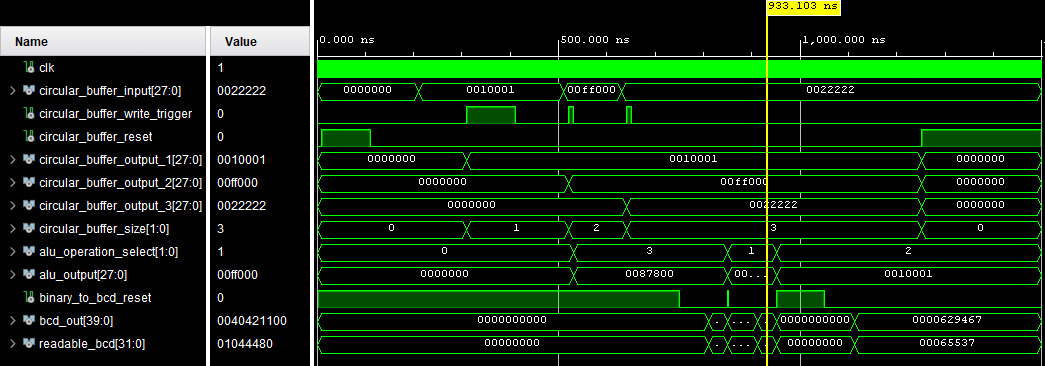
\includegraphics[width=0.99\textwidth]{thing.jpeg}
	\caption{Reaction statistic calculation testbench.}
	\label{fig:alu_testbench}
\end{figure}

The first 750 ns of testbench simulation show the three write operations to the circular buffer. The three circular buffer outputs change exactly as expected, with each write operation setting a new value. The ALU operation select is 3 at 700 ns, and the ALU output is 00878000, which is the correct hexadecimal representation of the average of the two values in the circular buffer when the operation was selected. The ALU operation is then set to 1 at approximately 850 ns, and the ALU outputs the correct maximum time of 00ff000. The final ALU operation is 2 at approximately 950 ns, and the ALU outputs the correct minimum time of 0010001. The binary-to-BCD converter is also triggered at 950 ns, and once the algorithm has completed, the BCD output is 00065537, which is the correct BCD representation of 0010001 in hexadecimal.

These waveforms indicated that the problem did not lie where expected, and that the problem must have been with the BCD-to-binary converter originally thought of as fault-free. Another testbench was created to test that converter, and, as expected, the converter did not convert correctly. This was rectified by modifying the multiplication factors of 10 from hexadecimal to binary. The fixed testbench waveform can be seen in Figure \ref{fig:correct_converter_tb}.

\begin{figure}[H]
	\centering
	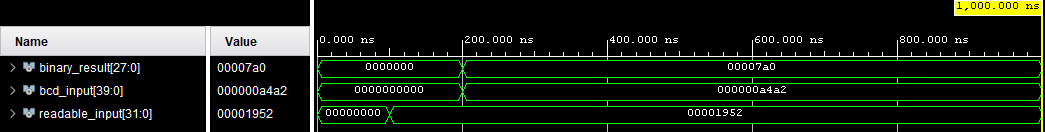
\includegraphics[width=0.99\textwidth]{WhatsApp Image 2025-05-08 at 16.13.24}
	\caption{Corrected BCD-to-binary converter testbench.}
	\label{fig:correct_converter_tb}
\end{figure}

These waveforms show the five-bit BCD and equivalent readable four-bit BCD inputs from the counter being correctly converted to binary. The readable BCD input is 00001952, which is equivalent to 00007a0, the hexadecimal representation of 1952.

\section{Design \& Implementation Problems}
% Design and/or Implementation problems (can be a separate section or part of the Conclusion): marks for describing problems encountered, and explaining approach to solving them.
% NB: Marks do not depend on whether problems were solved or not, but on the process used.
% 4 marks

One issue that arose during the development of the seven segment display component which mapped a BCD input to a combination of segments on a display to represent the BCD number was that the provided mappings did not represent the numbers correctly. The approach used to solve this was to first determine whether the BCD input or the mapping was incorrect. This was done by tying the BCD input to the green LEDs on the FPGA. This asserted that the BCD input was correct. To rectify the incorrect mappings, individual segments on a display were tied to the FPGA user switches. Combinations of switches were tested, and when the segments represented a number, the combination of switches was recorded as a BCD mapping.

However, once all the mappings were implemented, it was found that the countdown timer failed to display the decimal place values. Alteration of the countdown timer to display temporary digits instead of decimal place values revealed the countdown to be functional. Stepping through the code by hand revealed that, due to the use of the unfamiliar provided seven segment decoder, a line of code was overlooked that overwrote the decimal place value. Disabling this line of code allowed the countdown timer to show decimal place values.

A significantly unexpected issue that appeared during the testing of the finite state machine was deemed as the ``Schrodinger's States'' problem. This originated from the FSM running lines of code designed to change states even while they were commented out. To narrow down the source of the bug, the FSM was reduced to only what was necessary to run a simple reaction timer test without any ALU or error message. From there, states were slowly added back into the FSM and were tied to LEDs that would light up when the new states were activated. This showed additional issues in which an LED would trigger, but the state change wouldn't complete. With the suspicion that a race condition was in play, the issue was fixed by removing the FSM inputs from the sensitivity list of the FSM process, instead tying the process to a 10 kHz clock.

There were issues with the simulation software built into the Vivado toolchain. During the design and subsequent simulation of the BCD-to-binary numeric converter, the Vivado simulator would stop the simulation at the beginning of the numeric conversion, but would not give an error message to indicate an issue. The issue was narrowed down to being a problem with the simulator itself, as when a bitstream was generated for the whole system so that the converter could be tested on hardware, no issue was found.

Another issue that arose was regarding case sensitivity in VHDL. Although VHDL is not case sensitive, the constraints file required for the FPGA is. Early on during the project while developing the clock divider, the error message seen in Figure \ref{fig:error} was encountered. The approach to solving this problem was to ask the TAs in the lab what the message meant. However, they were unable to explain the meaning. From there, the clock divider code we wrote was thoroughly compared to the provided clock divider code, and every small difference tested to see if it repaired the error. This determined the issue to be the case of the clock input declared in entity of the \texttt{main} module, as lowercase had been used rather than uppercase. The correct case can be seen in Listing \ref{code:morecase}.

\begin{figure}[H]
	\centering
	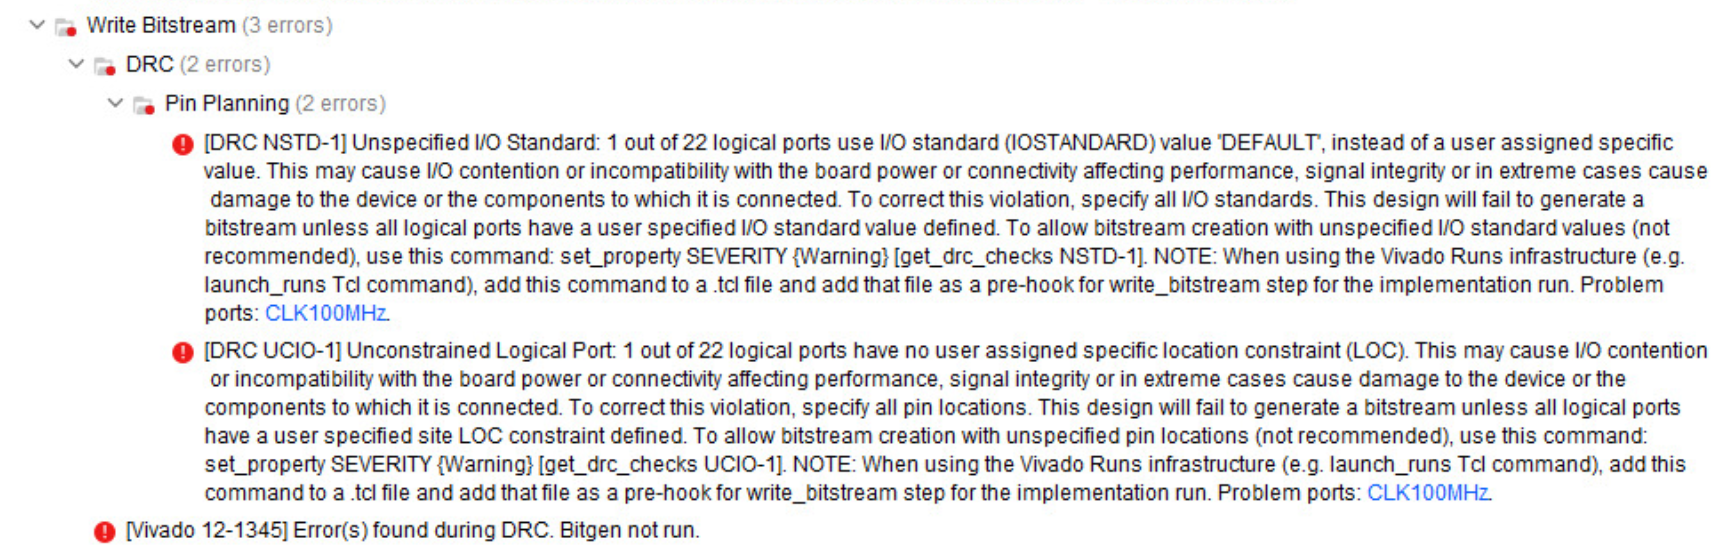
\includegraphics[width=0.99\textwidth]{error.png}
	\caption{Vivado error message regarding case sensitivity.}
	\label{fig:error}
\end{figure}

\section{Conclusion}
% Highlight any problems you encountered and how you solved them. Also discuss what you learned and give suggestions on how the project could be improved

% Project could be improved by allowing a non-fixed number of inputs to the ALU, so a more arbitrary number of results could be calculated
% Learnt how testbenches can be useful but have their limits as somethimes they have bugs which are not present when the code is run on hardware.

This project involved the development of a reaction stimulus test on an FPGA, utilizing VHDL and the Vivado toolchain to program the FPGA. The developed program enabled users to test their reaction speed to a stimulus that would occur at a random time, additionally being able to view the minimum, maximum, and average times of the last three tests.

The development process of the reaction stimulus test included a heavy focus on modularisation and code reuse. This is shown in the multiple uses of the 8x5-to-5 mux, and the self-contained ALU, timer, countdown, and error mdules. The use of modularisation significantly simplified the component assembly and debugging.

Numerous problems were encountered during the development process, both with the code and the Vivado development toolchain. Examples of code issues include the race condition found in the FSM, or the unusally small numbers returned by the BCD-to-binary numeric converter. Both issues were solved by narrowing down the range of operational code by either commenting out code, such as for the FSM, or by testing sections off the code in a testbench, as was done for the ALU module. The issue with the Vivado development toolchain was the code simulator refusing to run the BCD-to-binary converter without raising an exception that included an error message. This problem was solved by attempting to run the software on the FPGA, after which it was found to work without issue.

Further improvements to the reaction stimulus test could involve the addition of more display states, either by replacing the existing placeholder connections in the display select mux, or by chaining additional 8x5-to-5 muxes to increase the avaiable display inputs. The ALU could also be generalised to operate on any number of inputs as opposed to the hardcoded three inputs used for the project.

The project taught the group about FPGAs and VHDL styles, along with the advantages and disadvantages of each style. In addition, understanding was developed about the benefits and limitations of FPGAs, with the logic cells allowing for rapid calculation with simultaneous sets of signals, but could lead to unexpected race conditions.

% When developing the reaction timer, a number of problems were encountered. One of these involved the FSM changing states unexpectedly. To determine the cause of this problem, the FSM was simplified to a minimal working version, then slowly expanded. Another problem where the display module did not show the correct numbers was solved by creating a small program mapping switches to the BCD inputs of the display module. Both of these problems were solved by reducing the scope of the program, allowing the problem to be found without confusing things with extra complexity. This method, as well as the use of testbenches, was an effective way of finding problems in VHDL code.
%
% Modularity was a major strength, allowing new features to be integrated easily with the rest of the project, and simplifying module changes without other consequences. The modularity also reduced the effort needed to make changes such as increasing the number of bits in the BCD signals as there are less separate components in which the change needs to be made.
%
% The project could be expanded and improved by implementing the ALU in such a way that it could take an arbitrary number of inputs then calculate the average, maximum, and minimum of the inputs. Currently, the ALU is hardcoded to only accept three numbers and each of the input numbers needs its own signal going into the ALU module. This doesn't really fit with the modularity of the rest of the project as the ALU would need significant changes to work with more than three numbers.
%
\newpage
% There is no need to include a full code listing in your report as your code will be submitted via eng-git. However, reference to a code snippet in an appendix is quite appropriate. Formal citations to books, web articles, open source VHDL code and other sources should be listed in a reference section that uses the IEEE style and format.

\section{References}
\printbibliography

\newpage

\section{Appendix A: Code Listings}

\begin{code}
	\begin{minted}{vhdl}
  
    -- Define module IO
    entity counter_decade is
        Port ( EN_IN : in STD_LOGIC;
               RESET_IN : in STD_LOGIC;
               INCREMENT_IN : in STD_LOGIC;
               COUNT_OUT : out STD_LOGIC_VECTOR (3 downto 0);
               TICK_OUT : out STD_LOGIC);
    end counter_decade;

  \end{minted}
	\captionsetup{belowskip=0pt}
	\captionof{listing}{Entity naming example showing name post-fixes indicating data direction.}
	\label{code:entity_naming_convention}
\end{code}

\vspace*{1cm}

\begin{code}
	\begin{minted}{vhdl}
  entity clk_divider is
      Port ( CLK100MHZ_IN : in STD_LOGIC;
             UPPERBOUND_IN : in STD_LOGIC_VECTOR (27 downto 0);
             SLOWCLK_OUT : out STD_LOGIC);
  end clk_divider;

  architecture Behavioral of clk_divider is
    signal count: std_logic_vector (27 downto 0) := (others => '0');
    signal temp_clk: std_logic := '1';
    signal upperbound_half : std_logic_vector (27 downto 0);
  begin

  \end{minted}
	\captionsetup{belowskip=0pt}
	\captionof{listing}{Difference in case between port and internal signal type declarations.}
	\label{code:case_io}
\end{code}

\vspace*{1cm}

\begin{code}
	\begin{minted}{vhdl}
      entity counter_3b is
          Port ( CLK_IN : in STD_LOGIC;
                 COUNT_OUT : out STD_LOGIC_VECTOR (2 downto 0));
      end counter_3b;

      architecture Behavioral of counter_3b is
          signal count : std_logic_vector (2 downto 0) := (others => '0');
      begin

  \end{minted}
	\captionsetup{belowskip=0pt}
	\captionof{listing}{Difference in case between port and internal signal names.}
	\label{code:case}

\end{code}

\vspace*{1cm}

\begin{code}
	\begin{minted}{vhdl}
    library IEEE;
    use IEEE.STD_LOGIC_1164.ALL;
    
    entity multiplexer_8_1_4b is
        Port ( MUX_IN_0 : in STD_LOGIC_VECTOR (4 downto 0);
               MUX_IN_1 : in STD_LOGIC_VECTOR (4 downto 0);
               MUX_IN_2 : in STD_LOGIC_VECTOR (4 downto 0);
               MUX_IN_3 : in STD_LOGIC_VECTOR (4 downto 0);
               MUX_IN_4 : in STD_LOGIC_VECTOR (4 downto 0);
               MUX_IN_5 : in STD_LOGIC_VECTOR (4 downto 0);
               MUX_IN_6 : in STD_LOGIC_VECTOR (4 downto 0);
               MUX_IN_7 : in STD_LOGIC_VECTOR (4 downto 0);
               SELECT_IN : in STD_LOGIC_VECTOR (2 downto 0);
               MUX_OUT : out STD_LOGIC_VECTOR (4 downto 0));
    end multiplexer_8_1_4b;
    
    architecture Behavioral of multiplexer_8_1_4b is
    begin
        process (SELECT_IN, MUX_IN_0, MUX_IN_1, MUX_IN_2, MUX_IN_3,
                            MUX_IN_4, MUX_IN_5, MUX_IN_6, MUX_IN_7)
        begin
            case(SELECT_IN) is
                when "000" => MUX_OUT <= MUX_IN_0;
                when "001" => MUX_OUT <= MUX_IN_1;
                when "010" => MUX_OUT <= MUX_IN_2;
                when "011" => MUX_OUT <= MUX_IN_3;
                when "100" => MUX_OUT <= MUX_IN_4;
                when "101" => MUX_OUT <= MUX_IN_5;
                when "110" => MUX_OUT <= MUX_IN_6;
                when "111" => MUX_OUT <= MUX_IN_7;
            end case;
        end process;
    end Behavioral;
  \end{minted}
	\captionsetup{belowskip=0pt}
	\captionof{listing}{Generalised 8x5-to-5 mux.}
	\label{code:8x5_to_5_multiplexer}
\end{code}

\vspace*{1cm}

\begin{code}
	\begin{minted}{vhdl}
    entity bcd_8_to_binary is
        Port ( BCD_BUS_IN : in STD_LOGIC_VECTOR (39 downto 0);
              BINARY_OUT : out STD_LOGIC_VECTOR (27 downto 0));
    end bcd_8_to_binary;
  \end{minted}
	\captionsetup{belowskip=0pt}
	\captionof{listing}{BCD to binary converter entity definition.}
	\label{code:bcd_to_binary}
\end{code}

\vspace*{1cm}

\begin{code}
	\begin{minted}{vhdl}
    ff11: multiplexer_8_1_4b port map (MUX_IN_0 => encoded_reaction_time_digit,
                                       MUX_IN_1 => selected_alu_bcd_digit,
                                       MUX_IN_2 => selected_alu_bcd_digit,
                                       MUX_IN_3 => selected_alu_bcd_digit,
                                       MUX_IN_4 => encoded_error_text,
                                       MUX_IN_5 => encoded_display_placeholder,
                                       MUX_IN_6 => encoded_display_placeholder,
                                       MUX_IN_7 => encoded_dots,
                                       SELECT_IN => encoded_display_input_select,
                                       MUX_OUT => encoded_segment_data);
  \end{minted}
	\captionsetup{belowskip=0pt}
	\captionof{listing}{Module instantiation of output select 8x5-to-5 mux.}
	\label{code:output_select_mux_instantiation}
\end{code}

\vspace*{1cm}

\begin{code}

	\begin{minted}{vhdl}
    entity main is
      Port ( CLK100MHZ : in STD_LOGIC;
            AN : out STD_LOGIC_VECTOR (7 downto 0) := X"00";
            SEVEN_SEG : out STD_LOGIC_VECTOR (7 downto 0) := X"00";
            BTNC : in STD_LOGIC;
            BTNR : in STD_LOGIC;
            BTNL : in STD_LOGIC;
            BTNU : in STD_LOGIC;
            BTND : in STD_LOGIC);  
    end main;
  \end{minted}
	\captionsetup{belowskip=0pt}
	\captionof{listing}{Correct case of port names in entity definition.}
	\label{code:morecase}
\end{code}

\newpage

\section{Appendix B: Testbench \& Waveforms}

\vspace*{1cm}
\begin{code}
	\begin{minted}{vhdl}
----------------------------------------------------------------------------------
-- Engineers: Michael Brown, Philip Brand
-- Create Date: 25.04.2025 02:04:31
-- Module Name: alu_setup_tb - Behavioral
-- Project Name: ALU Setup Test Bench 
-- Description: Tests the alu, circular_buffer, and binary_to_bcd_8 modules.
-- Additional Comments: Used to test the more complex parts of the 
-- reaction statistic calculations.
----------------------------------------------------------------------------------

library IEEE;
use IEEE.STD_LOGIC_1164.ALL;

entity alu_setup_tb is
--  Port ( );
end alu_setup_tb;

architecture Behavioral of alu_setup_tb is
    signal circular_buffer_output_1 : std_logic_vector (27 downto 0) := (others => '0');
    signal circular_buffer_output_2 : std_logic_vector (27 downto 0) := (others => '0');
    signal circular_buffer_output_3 : std_logic_vector (27 downto 0) := (others => '0');
    signal circular_buffer_input : std_logic_vector (27 downto 0) := (others => '0');
    signal circular_buffer_size : std_logic_vector (1 downto 0) := (others => '0');
    signal alu_operation_select : std_logic_vector (1 downto 0) := (others => '0');
    signal circular_buffer_write_trigger : std_logic := '0';
    signal circular_buffer_reset : std_logic := '0';
    signal clk : std_logic := '0';
    signal binary_to_bcd_reset : std_logic := '0';
    signal bcd_out : std_logic_vector (39 downto 0) := (others => '0');
    signal bcd_out_expanded : std_logic_vector (31 downto 0) := (others => '0');
    signal alu_output : std_logic_vector (27 downto 0) := (others => '0');
    
    component alu is
        Port ( NUM_1_IN, NUM_2_IN, NUM_3_IN : in STD_LOGIC_VECTOR (27 downto 0);
               BUFFER_SIZE_IN, OPERATION_SELECT_IN : in STD_LOGIC_VECTOR (1 downto 0);
               OUTPUT_OUT : out STD_LOGIC_VECTOR (27 downto 0));
    end component alu;

    component circular_buffer is
        Port ( NUMBER_IN : in STD_LOGIC_VECTOR (27 downto 0);
               NUMBER_1_OUT, NUMBER_2_OUT, NUMBER_3_OUT : out STD_LOGIC_VECTOR (27 downto 0);
               BUFFER_SIZE_OUT : out STD_LOGIC_VECTOR (1 downto 0);
               RESET_IN, WRITE_TRIGGER_IN : in STD_LOGIC);
    end component circular_buffer;

    component binary_to_bcd_8 is
        Port ( CLK_IN : IN  std_logic;
               RESET_IN : IN  std_logic;
               BINARY_IN : IN  std_logic_vector(27 downto 0);
               BCD_8_DIGIT_OUT : OUT std_logic_vector (39 downto 0) := (others => '0'));
    end component binary_to_bcd_8;

begin
    ff0: alu port map ( NUM_1_IN => circular_buffer_output_1,
                        NUM_2_IN => circular_buffer_output_2,
                        NUM_3_IN => circular_buffer_output_3,
                        BUFFER_SIZE_IN => circular_buffer_size,
                        OPERATION_SELECT_IN => alu_operation_select,
                        OUTPUT_OUT => alu_output);
    
    ff1: circular_buffer port map ( NUMBER_IN => circular_buffer_input,
                                    NUMBER_1_OUT => circular_buffer_output_1,
                                    NUMBER_2_OUT => circular_buffer_output_2,
                                    NUMBER_3_OUT => circular_buffer_output_3,
                                    BUFFER_SIZE_OUT => circular_buffer_size,
                                    RESET_IN => circular_buffer_reset,
                                    WRITE_TRIGGER_IN => circular_buffer_write_trigger);

    ff2: binary_to_bcd_8 port map ( CLK_IN => clk,
                                    RESET_IN => binary_to_bcd_reset,
                                    BINARY_IN => alu_output,
                                    BCD_8_DIGIT_OUT => bcd_out);
    
    bcd_out_expanded(31 downto 28) <= bcd_out(38 downto 35);
    bcd_out_expanded(27 downto 24) <= bcd_out(33 downto 30);
    bcd_out_expanded(23 downto 20) <= bcd_out(28 downto 25);
    bcd_out_expanded(19 downto 16) <= bcd_out(23 downto 20);
    bcd_out_expanded(15 downto 12) <= bcd_out(18 downto 15);
    bcd_out_expanded(11 downto 8) <= bcd_out(13 downto 10);
    bcd_out_expanded(7 downto 4) <= bcd_out(8 downto 5);
    bcd_out_expanded(3 downto 0) <= bcd_out(3 downto 0);

    simulation_clk : process
    begin
        wait for 1ns;
        clk <= '1';
        wait for 1ns;
        clk <= '0';
    end process;
    
    simulation : process
    begin
        binary_to_bcd_reset <= '1';
        wait for 10ns;
        circular_buffer_reset <= '1';
        circular_buffer_input <= X"0000000";
        wait for 100ns;
        circular_buffer_reset <= '0';
        wait for 100ns;
        circular_buffer_input <= X"0010001";
        binary_to_bcd_reset <= '1';
        wait for 100ns;
        circular_buffer_write_trigger <= '1';
        wait for 100ns;
        circular_buffer_write_trigger <= '0';
        wait for 100ns;
        circular_buffer_input <= X"00FF000";
        wait for 10ns;
        circular_buffer_write_trigger <= '1';
        wait for 10ns;
        alu_operation_select <= "11";
        circular_buffer_write_trigger <= '0';
        wait for 100ns;
        circular_buffer_input <= X"0022222";
        wait for 10ns;
        circular_buffer_write_trigger <= '1';
        wait for 10ns;
        circular_buffer_write_trigger <= '0';
        wait for 100ns;
        binary_to_bcd_reset <= '0';
        wait for 100ns;
        binary_to_bcd_reset <= '1';
        alu_operation_select <= "01";
        wait for 1ns;
        binary_to_bcd_reset <= '0';
        wait for 100ns;
        binary_to_bcd_reset <= '1';
        alu_operation_select <= "10";
        wait for 100ns;
        binary_to_bcd_reset <= '0';
        wait for 200ns;
        circular_buffer_reset <= '1';
        wait for 100000ns;
    end process;

  \end{minted}
	\captionsetup{belowskip=0pt}
	\captionof{listing}{Testbench for ALU, circular buffer, and BCD to binary converter.}
	\label{code:alu_testbench}
\end{code}

\vspace*{1cm}

The waveform associated with the testbench in Listing \ref{code:alu_testbench} can be seen in Figure \ref{fig:alu_testbench_2}.

\begin{figure}[H]
	\centering
	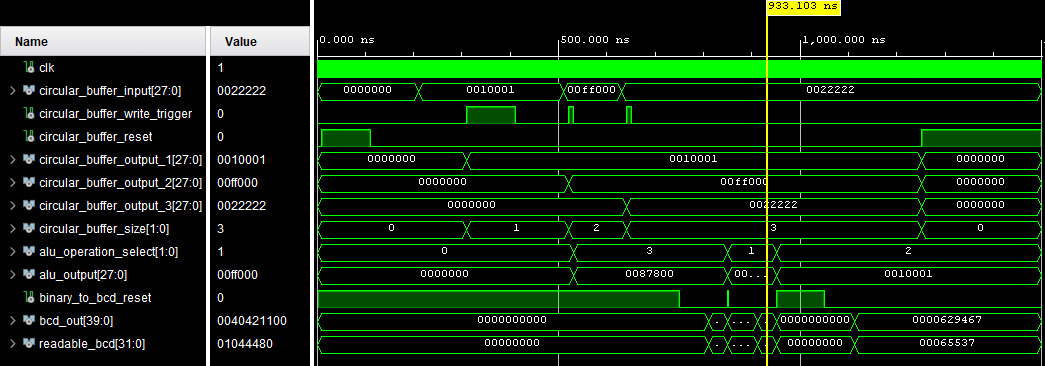
\includegraphics[width=0.99\textwidth]{thing.jpeg}
	\caption{Reaction statistic calculation testbench.}
	\label{fig:alu_testbench_2}
\end{figure}

\newpage

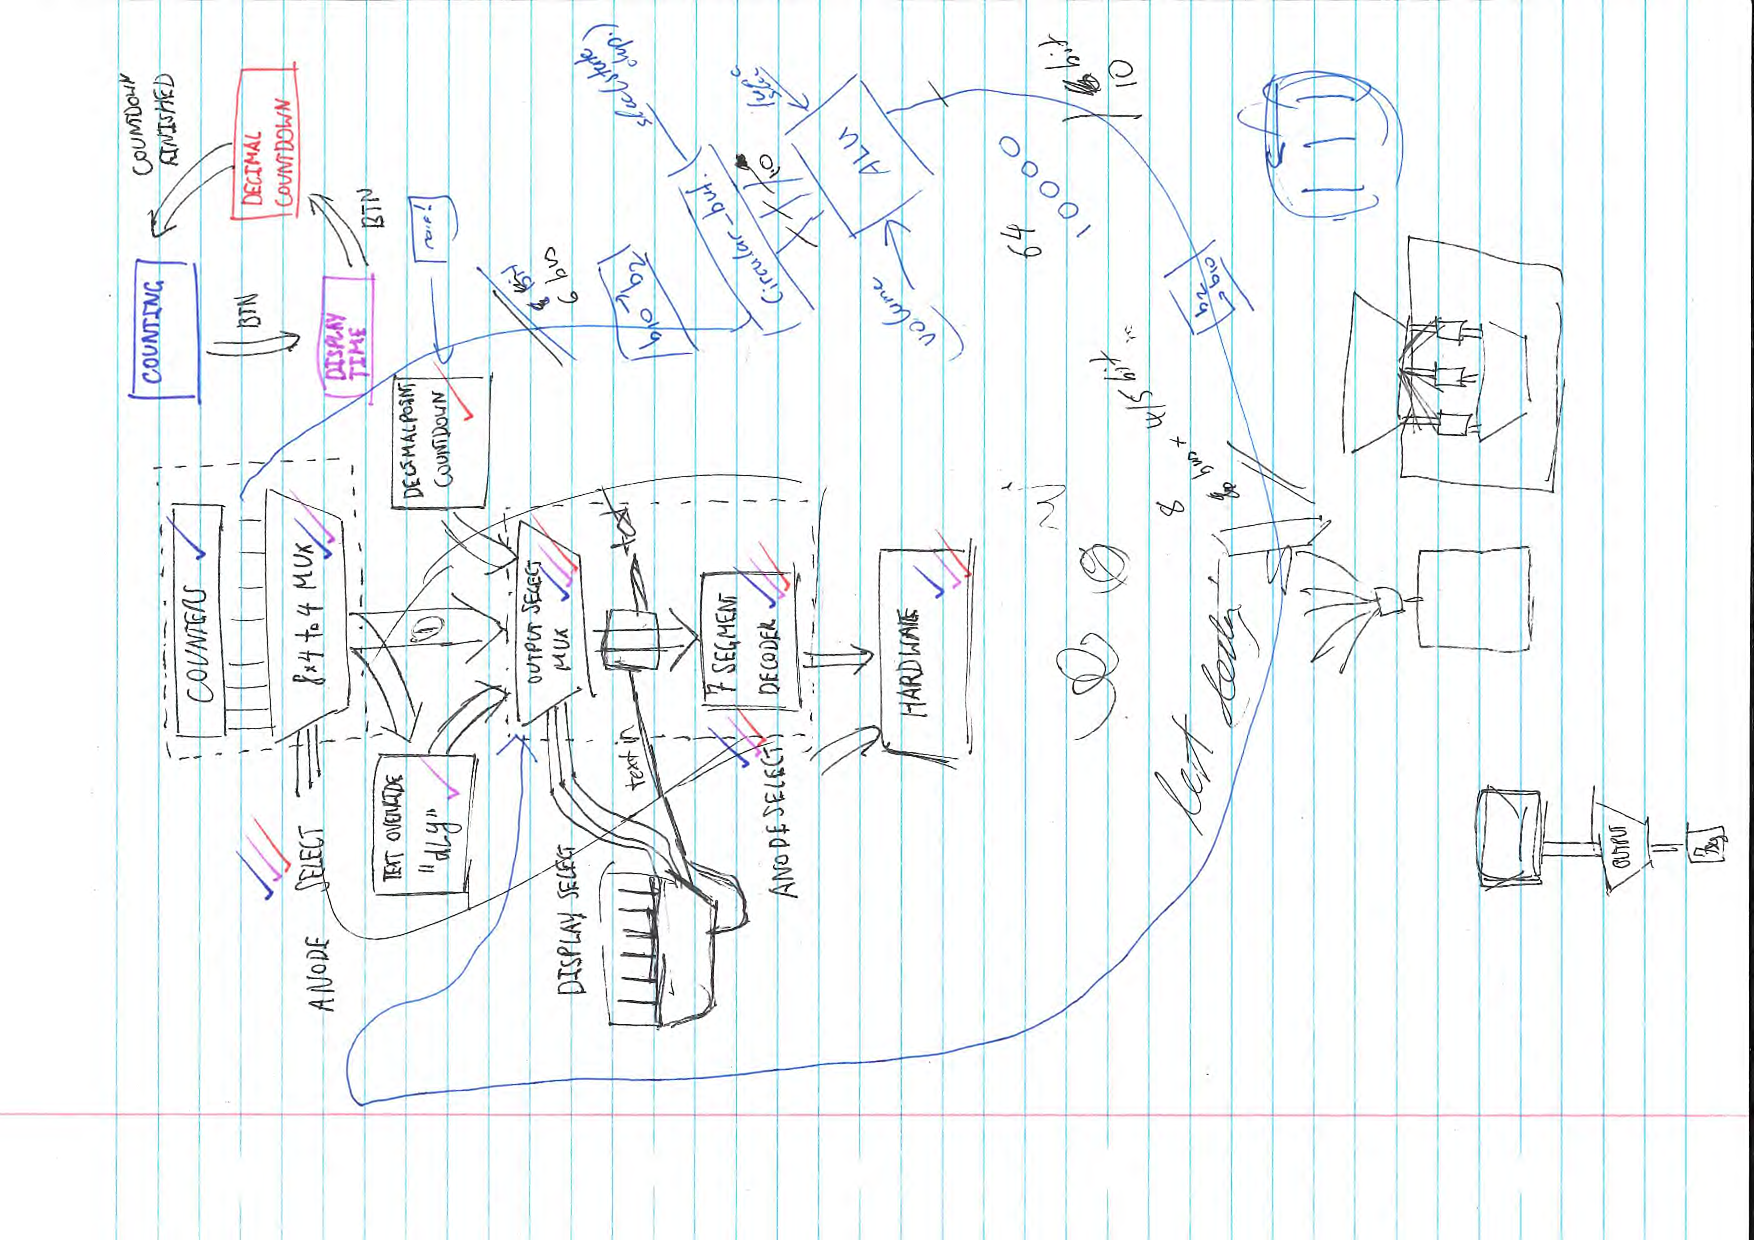
\includepdf[pages=-, pagecommand={\section{Appendix C: Program Structure Brainstorm Diagram}}, rotate=-90, width=0.85\textwidth]{../figures/diagram.pdf}
\end{document}

